\section{Monte Carlo Radiation Transport}
\label{sec:bg:mc}

Blah blah blah.. background information in a section with equations and a reference to \ac{mcnp} \cite{mcnp5-theory}.

\begin{equation}\label{bg:eq:std}
\begin{split}
	\sigma_x^2 &= \frac{\sum \left(x_i - \bar{x}\right)^2}{N-1} \\
	\sigma_{\bar{x}}^2 &= \frac{\sigma_x^2}{N}
\end{split}
\end{equation}

\begin{equation}\label{bg:eq:relerror}
	R = \frac{\sigma_{\bar{x}}}{\bar{x}}
\end{equation}

Another quantity of interest to measure computational performance is the figure of merit, defined by Equation \ref{bg:eq:fom} where $t_{proc}$ is the processor time required 
for the
simulation \cite{mcnp5-theory}. It is desirable to have a high figure of merit meaning there is low 
relative error and low processor time. 

\begin{equation}\label{bg:eq:fom}
	FOM = \frac{1}{R^2 t_{proc}}
\end{equation}

\subsection{Variance Reduction}
\label{sec:bg:vr}

As described in Section \ref{sec:bg:mc}, some Monte Carlo radiation 
transport problems must employ variance reduction techniques to lower the 
variance $\sigma_{\bar{x}}^2$.

Here is an example figure with a caption (see Figure \ref{fig:prep:isosurf-mesh}).
\begin{figure}[h!]
\centering
	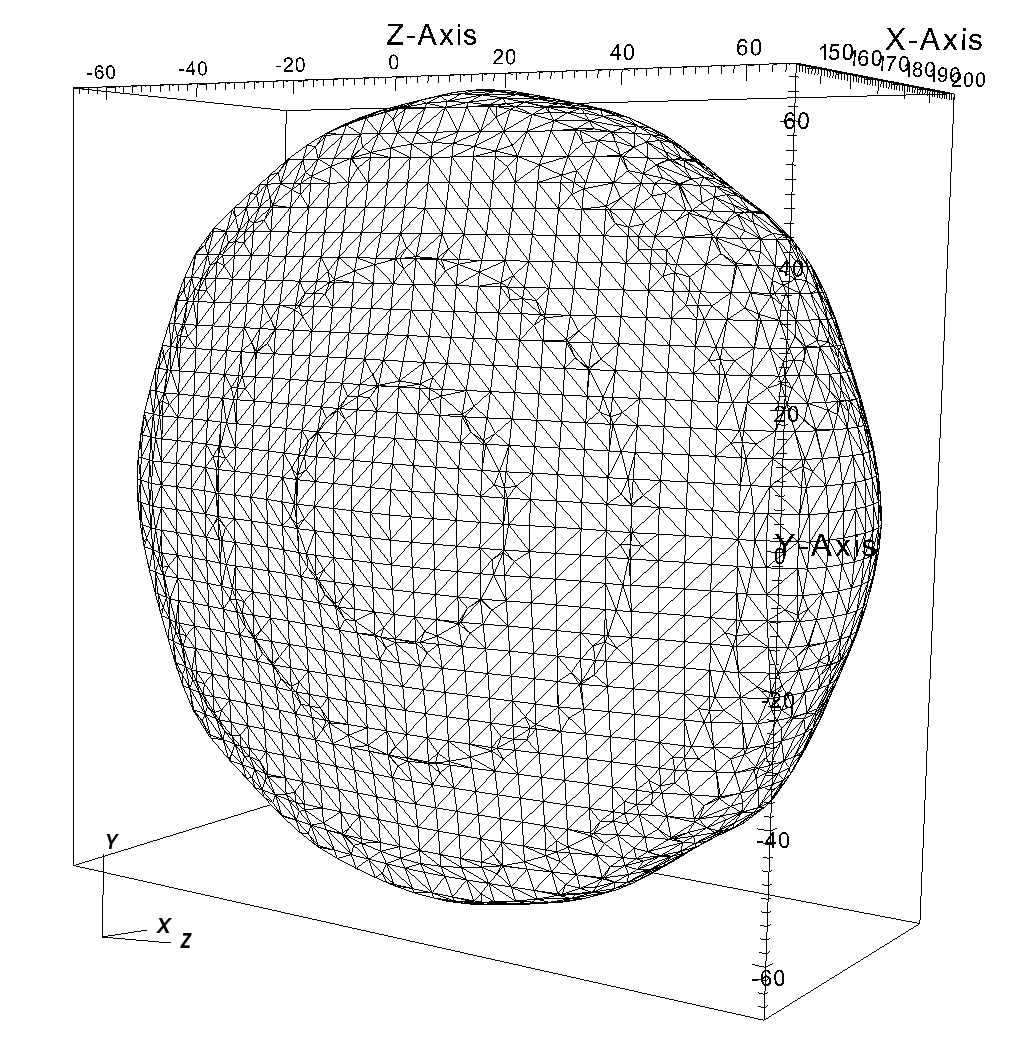
\includegraphics[width=.5\textwidth]{./content/background/example-isosurf.png}
	\caption[Example VisIt surface mesh]{Example surface mesh generated by VisIt of the volume between two isosurfaces.
	\label{fig:prep:isosurf-mesh}}
\end{figure}

Here is an example table to appear in list of tables (see Table \ref{tab:toy:zvalue}). It also uses ``num" for formatting numbers.

\begin{table}[h]
\centering
\caption{Neutron Flux Z-values} \label{tab:toy:zvalue}
	\begin{tabular}{| c | c | c |}
	\hline
	\textbf{Reference Mesh} & \textbf{Comparison Mesh} & \% \textbf{voxels with $z \leq 2\sigma$} \\
	\hline
	Analog & Cartesian WW Mesh & \num{98.34}\% \\
	\hline
	Analog & WWIG & \num{98.09}\% \\
	\hline
	Cartesian WW Mesh & WWIG & \num{98.13}\% \\
	\hline
	\end{tabular}
\end{table}